\documentclass[dvipdfmx]{jsarticle}
\usepackage{graphics}
\usepackage{amsmath}
\usepackage{amssymb}
\usepackage{amsthm}
\usepackage{mathtools}
\usepackage{ascmac}
\usepackage{bm}
\usepackage{url}
\usepackage{txfonts}
\usepackage{color}
\usepackage{tikz}
% \usepackage{docmute}    %パッケージのダウンロードが必要
\usepackage{tikz}
\usetikzlibrary{calc}
\usetikzlibrary{intersections}

\begin{document}
    \section{ベクトル方程式の導入}
    原点を始点とし,成分が(1,0)となるベクトル \(\vec{x}\)をとる.するとxy平面において,x軸上の任意の点は \(t\vec{x},(t\text{は実数})\)というベクトルで表現できる.これはx軸という直線がベクトルと実数の積で表現されたということができる.このように,空間上の点や直線,面などをベクトルと実数で表すのがベクトル方程式だ.以下,代表的なベクトル方程式を紹介する.

    \section{直線のベクトル方程式}
    \subsection{位置と方向1}

    直線のベクトル方程式で必要なのは,直線の進む方向(傾き)と直線の位置(直線の通過する1点)だ.1次関数が傾きとy切片で決定することに似ている.定点Oをとり,点A,Bを通る直線を考えると,そのベクトル方程式 \(\vec{p}\)\footnote{ベクトル方程式を考えるときに,表現する図形上の点をPとし,そのベクトルを \(\vec{p}\)とするのは慣習である.}は
    \[
    \vec{p}=\vec{a} + t(\vec{b}-\vec{a})\qquad t:\text{実数}
    \]
    となる(図\ref{tikz_vector_equation_line1}).

    \begin{figure}[htbp]\centering
        \begin{tikzpicture}\large
            \coordinate (o) at (0,0);
            \coordinate (a) at (-1,2);
            \coordinate (b) at (2,3);

            \fill (o)node[below]{O} circle (2pt);
            \fill (a)node[above]{A} circle (2pt);
            \fill (b)node[above]{B} circle (2pt);

            \draw ($(a)  -(b)+(a)$) -- ($(a) + 2*(b) - 2*(a)$);

            \draw[red,thick,->](o)--node[left]{\(\vec{a}\)}(a);
            \draw[red,thick,->](a)--node[below]{\(t(\vec{b}-\vec{a})\)}($1/3*(a)+2/3*(b)$);
            \fill[red] ($1/3*(a)+2/3*(b)$)node[above]{P} circle(2pt);

        \end{tikzpicture}
        \caption{直線のベクトル方程式1}
        \label{tikz_vector_equation_line1}
    \end{figure}

    \(t\)を自由に変化させることで直線AB上を点Pが動くことがわかる.ここからは直線のベクトル方程式を一般化する.まずは直線の位置を表す部分だ. \(\vec{a}\)によって直線と点Oの位置関係が決定している.だが,これは直線上の1点であれば何でもよい.図のようなベクトルを考え,
    \[
    \vec{p}=\vec{c} + t(\vec{b}-\vec{a})\qquad t:\text{実数}
    \]
    としても良い.

    \begin{figure}[htbp]\centering
        \begin{tikzpicture}\large
            \coordinate (o) at (0,0);
            \coordinate (a) at (-1,2);
            \coordinate (b) at (2,3);
            \coordinate (c) at ($5/4*(a)-1/4*(b)$);

            \fill (o)node[below]{O} circle (2pt);
            \fill (a)node[above]{A} circle (2pt);
            \fill (b)node[above]{B} circle (2pt);
            \fill (c)node[above]{C} circle (2pt);

            \draw ($(a)  -(b)+(a)$) -- ($(a) + 2*(b) - 2*(a)$);

            \draw[red,thick,->](o)--node[left]{\(\vec{c}\)}(c);
            \draw[red,thick,->](c)--node[below]{\(t(\vec{b}-\vec{a})\)}($1/3*(a)+2/3*(b)$);
            \fill[red] ($1/3*(a)+2/3*(b)$)node[above]{P} circle(2pt);

        \end{tikzpicture}
        \caption{直線のベクトル方程式2}
        \label{tikz_vector_equation_line1_sub1}
    \end{figure}

    もちろん,直線の位置を示すベクトルが \(\vec{a}\)から \(\vec{c}\)に変わっているので,同じ点Pを表現しようと思うと, \(t\)の値が変わる.しかし,直線を表現しているという点では何ら変化はない.


    次に一般化するのは直線の方向を示すベクトルだ.今の例では \(\vec{b}-\vec{a}\)が方向を示すベクトルとなっているが,これは実数倍で自由\footnote{自由とは,変更が可能であるということである. \(t(\vec{b}-\vec{a})=t/2\cdot 2(\vec{b}-\vec{a})\)であるから方向を表すベクトルを \(2(\vec{b}-\vec{a})\)に変更しても問題はない.}だ.そこで方向を示すベクトルは \(\vec{b}-\vec{a}\)に平行な何らかのベクトル \(\vec{d}\)であるとする.

    以上から一般的な直線のベクトル方程式は
    \begin{equation}
        \vec{p}=\vec{c}+t\vec{d}\qquad t:\text{実数}
        \label{eq_vector_equation_line1}
    \end{equation}
    とすることができる\footnote{変化しない定ベクトルをconstant vector,方向ベクトルをdirection vectorと呼び,そこから \(\vec{c},\vec{d}\)としていたりもする.}.直線のベクトル方程式を求めるとは, \(\vec{c},\vec{d}\)を求めることである.もちろん2次元,3次元で同じように扱える公式である.

    \subsection{位置と方向2}
    前項では方向を直接に表現していた. \(\vec{d}\)によって方向を決定し \(t\)倍していた.ベクトルの世界では"同じ方向"と同じくらい特殊な方向の関係がある.それは"垂直"であり,本項では直線の方向を,その法線で与えられている場合を考える.

    図\ref{tikz_vector_equation_line2}のように法線ベクトル \(\vec{n}\)\footnote{法線ベクトルはnormal vectorと呼ぶ.そのため法線ベクトルは \(\vec{n}\).}と,直線上の一点が与えられているとする.すると直線上の任意の点Pをとることで次の式を立てることができる.
    \begin{equation}
        \vec{n}\cdot(\vec{p}-\vec{c})=0
        \label{eq_vector_equation_line2}
    \end{equation}
    これがベクトル方程式なのだ.式\eqref{eq_vector_equation_line1}とは異なり,変数 \(t\)がない.そのため,直線上の1点を決定することはできない.だが, \(\vec{p}\)は直線上のすべての点になり得ることになり,直線全体を表すベクトル方程式であるということができる.

    \begin{figure}[htbp]\centering
        \begin{tikzpicture}\large
            \coordinate (o) at (0,0);
            \coordinate (c) at (-1,2);
            \coordinate (p) at (2,3);
            \coordinate (n) at ($(c)!0.5!(p)$);

            \fill (o)node[below]{O} circle (2pt);
            \fill (a)node[above]{A} circle (2pt);

            \draw ($(c)!-1!(p)$)--($(c)!2!(p)$);
            \draw[red,thick,->] (n)--node[above right]{\(\vec{n}\)}($(n)!1cm!90:(p)$);
            \draw[red,thick,->] (c)--node[below right]{\(\vec{p}-\vec{c}\)}(p)node[above]{P};

        \end{tikzpicture}
        \caption{直線のベクトル方程式3}
        \label{tikz_vector_equation_line2}
    \end{figure}

    理解が難しいのは \(\vec{p}\)が決定しないからだ.ベクトル方程式というのは,図形のある1点をPとしたときに
    \[
    \vec{p}=(\text{条件式})
    \]
    という風に点を決定するものではなく,図形のすべての点Pに対して \(\vec{p}\)が満たす式である.このことを念頭に話を進める.

    \section{円のベクトル方程式}
    \subsection{中心と半径}
    円とは,半径から等距離に存在する点の集合だ.そこで円の中心を示す位置ベクトルを \(\vec{c}\),半径を \(r\)とすると,円周上のすべての \(\vec{p}\)は
    \begin{equation}
        |\vec{p}-\vec{c}|=r
        \label{eq_vector_equation_circle1}
    \end{equation}
    を満たす.これが円のベクトル方程式なのだ.図\ref{tikz_vector_equation_circle1}がその参考となる図である.

    \begin{figure}[htbp]\centering
        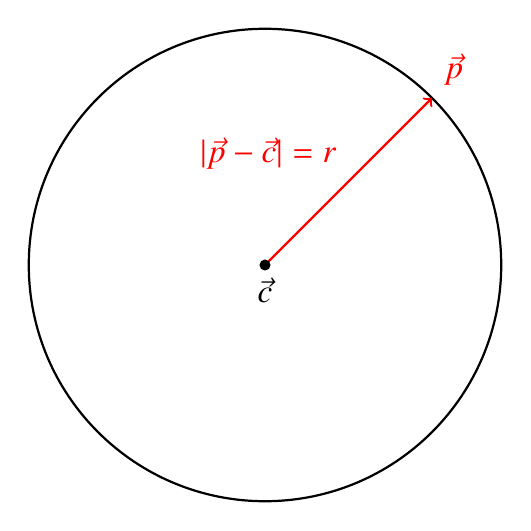
\begin{tikzpicture}\large
            \coordinate (o) at (0,0);
            \coordinate (p) at (45:3);

            \draw[thick] (o)node[below]{\(\vec{c}\)} circle[radius=3];
            \draw[red,thick,->](o)--node[above left]{\(|\vec{p}-\vec{c}|=r\)}(p)node[above right]{\(\vec{p}\)};
            \fill (o) circle (2pt);

        \end{tikzpicture}
        \caption{円のベクトル方程式}
        \label{tikz_vector_equation_circle1}
    \end{figure}

    \subsection{直径}
    線分ABを直径とする円を考える.この場合のベクトル方程式を考えるときに利用するのは,直径の円周角が90度であることだ.直角であればベクトルの内積が0になるので,ここからベクトル方程式を立てることができる.

    線分の両端の位置ベクトルを \(\vec{a},\vec{b}\)とすると,円のベクトル方程式は
    \begin{equation}
        (\vec{p}-\vec{a})\cdot(\vec{p}-\vec{b})=0
        \label{eq_vector_equation_circle2}
    \end{equation}
    となる.次のようなイメージとなる(図\ref{tikz_vector_equation_circle2}).

    \begin{figure}[htbp]\centering
        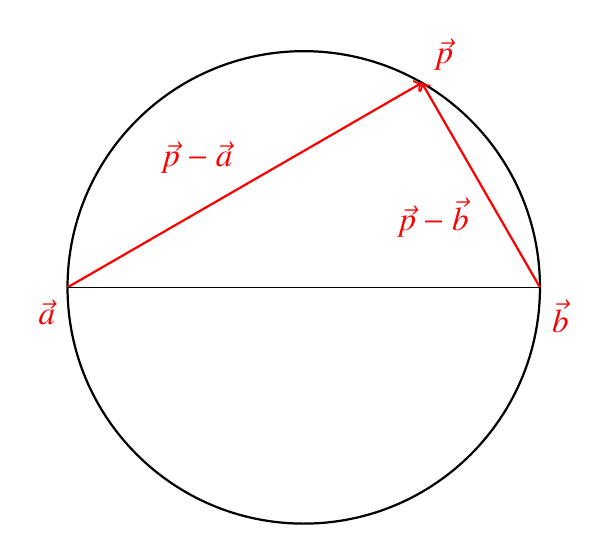
\begin{tikzpicture}\large
            \coordinate (o) at (0,0);
            \coordinate (a) at (-3,0);
            \coordinate (b) at (3,0);
            \coordinate (p) at (60:3);

            \draw[thick](o)circle[radius=3];
            \draw[red,thick,->](a)node[below left]{\(\vec{a}\)}--node[above left]{\(\vec{p}-\vec{a}\)}(p)node[above right]{\(\vec{p}\)};
            \draw[red,thick,->](b)node[below right]{\(\vec{b}\)}--node[below left]{\(\vec{p}-\vec{b}\)}(p);

            \draw (a)--(b);
        \end{tikzpicture}
        \caption{円のベクトル方程式}
        \label{tikz_vector_equation_circle2}
    \end{figure}

    点PがもしA,Bと一致しても式\eqref{eq_vector_equation_circle2}を満たすので心配はない.2つの円のベクトル方程式を紹介したが,どちらも円周上の1点を決定するものではない.

    \section{平面のベクトル方程式}
    \subsection{位置と平面}
    一次独立な2つのベクトルがあれば,その2つのベクトルが属する平面の任意の点を示すことができる.これは前章で扱った内容だ.そして,それと平面の位置を決定する要素があれば,3次元空間に1つの平面を決定することができる.

    今の表現は難解なので,具体例を示す.図のように,基準となる定点Oと3点A,B,Cをとる.すると,3点A,B,Cによって決定する平面のベクトル方程式は次のようになる.
    \[
    \vec{p}=\vec{a} + s(\vec{b}-\vec{a})+t(\vec{c}-\vec{a})\qquad s,t:\text{実数}
    \]

    \begin{figure}[htbp]\centering
        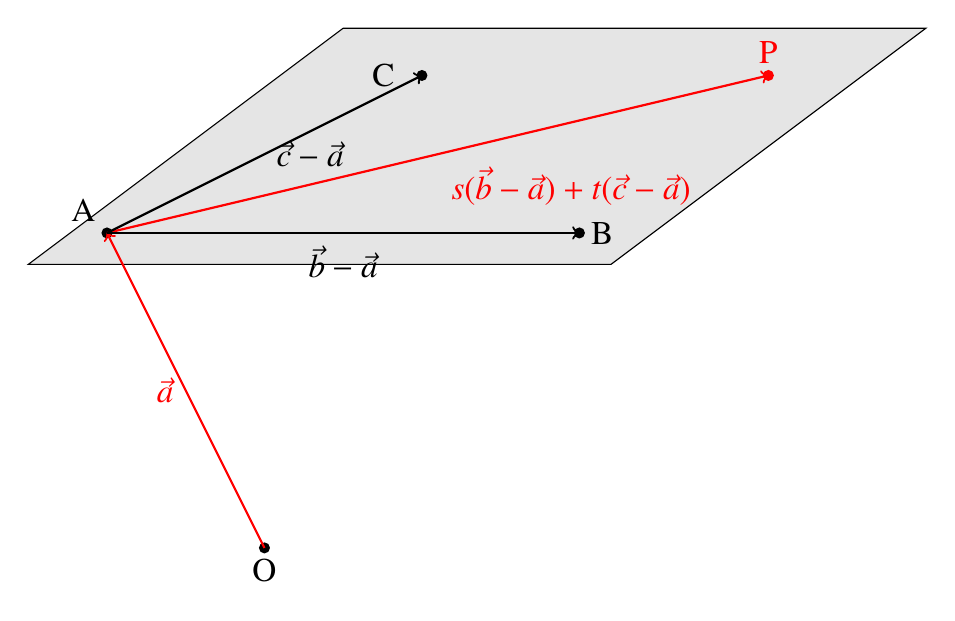
\begin{tikzpicture}[scale=2]\large
            \coordinate (o) at (0,0);
            \coordinate (a) at (-1,2);
            \coordinate (b) at (2,2);
            \coordinate (c) at (1,3);
            \coordinate (p) at (3.2,3);

            \filldraw[fill=black!10,draw=black,thin] (-1.5,1.8)--(2.2,1.8)--(4.2,3.3)--(0.5,3.3)--cycle;
            \fill (o)node[below]{O} circle(1pt);
            \fill (a)node[above left]{A} circle(1pt);
            \fill (b)node[right]{B} circle(1pt);
            \fill (c)node[left=2mm]{C} circle(1pt);
            \fill[red] (p)node[above]{P} circle(1pt);

            \draw[red,thick,->](o)--node[left]{\(\vec{a}\)}(a);
            \draw[red,thick,->](a)--node[below right]{\(s(\vec{b}-\vec{a})+t(\vec{c}-\vec{a})\)}(p);

            \draw[thick,->](a)--node[below]{\(\vec{b}-\vec{a}\)}(b);
            \draw[thick,->](a)--node[right]{\(\vec{c}-\vec{a}\)}(c);
        \end{tikzpicture}
        \caption{平面のベクトル方程式1}
        \label{tikz_vector_equation_plane1}
    \end{figure}

    直線のベクトル方程式と同じように一般化を考える.面の一点を示す位置ベクトルを \(\vec{c}\)\footnote{図\ref{tikz_vector_equation_plane1}の \(\vec{c}\)とは別物.定ベクトル.}とし,さらに示したい平面に属する一次独立はベクトルの組を \(\vec{k},\vec{l}\)とすると,平面のベクトル方程式は,
    \begin{equation}
        \vec{p} =\vec{c} +s\vec{k}+t\vec{l}\qquad s,t:\text{実数}
        \label{eq_vector_equation_plane1}
    \end{equation}
    となる.

    \subsection{位置と法線}
    直線と同様で,平面のベクトル方程式でも法線ベクトルを考えることができる.面の法線とは面のいかなる線分に対しても垂直な直線のことである.ここから法線ベクトル \(\vec{n}\)は面に属する一次独立な2本のベクトルの両方と垂直なベクトルとすることができる.法線ベクトルと,平面上の1点 \(\vec{c}\)によってベクトル方程式は
    \begin{equation}
        \vec{n}\cdot (\vec{p}-\vec{c})=0
        \label{eq_vector_equation_plane2}
    \end{equation}
    となる(図\ref{tikz_vector_equation_plane2}).

    \begin{figure}[htbp]\centering
        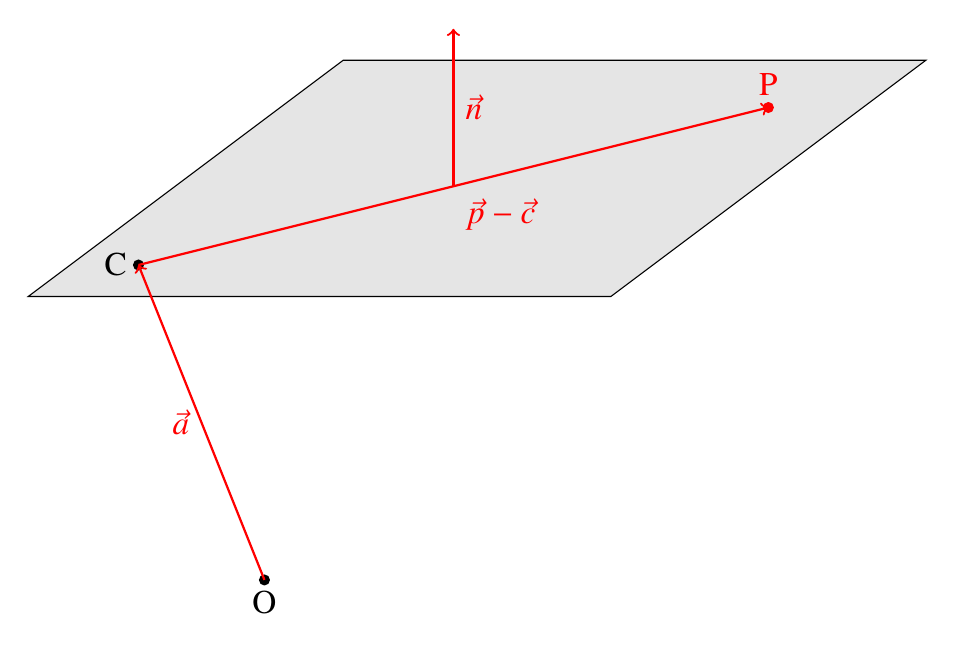
\begin{tikzpicture}[scale=2]\large
            \coordinate (o) at (0,0);
            \coordinate (c) at (-0.8,2);
            \coordinate (p) at (3.2,3);

            \filldraw[fill=black!10,draw=black,thin] (-1.5,1.8)--(2.2,1.8)--(4.2,3.3)--(0.5,3.3)--cycle;
            \fill (o)node[below]{O} circle(1pt);
            \fill (c)node[left]{C} circle(1pt);
            \fill[red] (p)node[above]{P} circle(1pt);

            \draw[red,thick,->](o)--node[left]{\(\vec{a}\)}(c);
            \draw[red,thick,->](c)--node[below right]{\(\vec{p}-\vec{c}\)}(p);

            \draw[red ,thick,->]($(c)!0.5!(p)$)--node[right]{\(\vec{n}\)}($(c)!0.5!(p) + (90:1)$);

        \end{tikzpicture}
        \caption{平面のベクトル方程式2}
        \label{tikz_vector_equation_plane2}
    \end{figure}

    平面上のすべての \(\vec{p}\)で式\eqref{eq_vector_equation_plane2}が成立する.ことからこれはベクトル方程式である.

    \section{球のベクトル方程式}
    これは円のベクトル方程式を3次元に拡張したものだ.中心の座標を \(\vec{c}\),半径を \(r\)とすると,
    \begin{equation}
        |\vec{p}-\vec{c}|=r
        \label{eq_vector_equation_ball1}
    \end{equation}
    となる.これは式\eqref{eq_vector_equation_circle1}と全く同じ式だ.

    さらに,球の直径の両端がわかるときにベクトル方程式は式\eqref{eq_vector_equation_circle2}と同じで,
    \begin{equation}
        (\vec{p}-\vec{a})\cdot(\vec{p}-\vec{b})=0
        \label{eq_vector_equation_ball2}
    \end{equation}
    となる.

    \section{ベクトル方程式と座標系}
    ベクトル方程式において,そのベクトルの成分が明らかなとき,座標系の関数に直すことができる.媒介変数表示というものの理解が必要だ.
    \subsection{直線のベクトル方程式と座標系}
    直線のベクトル方程式である式\eqref{eq_vector_equation_line1}において,
    \[
    \begin{cases}
        \vec{c}&=(1,2)\\
        \vec{d}&=(3,2)
    \end{cases}
    \]
    とする.直線上の点を \(\vec{p}=(x,y)\)とすると,ベクトル方程式から
    \begin{align*}
        (x,y)&= (1,2)+t(3,2)\\
        \Rightarrow &\begin{cases}
            x&= 3t+1\\
            y&=2t+2
        \end{cases}
    \end{align*}
    と分かる.これは媒介変数 \(t\)の媒介変数表示である.さらに,媒介変数を消去することで,
    \[
    2x-3y=4\Rightarrow y=\frac{2}{3}x- \frac{4}{3}
    \]
    を得る.これで直線のベクトル方程式を1次関数にすることができた.

    次は式\eqref{eq_vector_equation_line2}の形のベクトル方程式を求める.法線ベクトル \(\vec{n}\)は \(\vec{d}\)に垂直なベクトルとして与えられる.そこから,内積を計算することで求めることができる.そのほかにも求める方法があり,直線の方程式
    \[
    2x-3y=-4
    \]
    から, \(x,y\)の係数を取り出すことで \(\vec{n}=(2,-3)\)とすることもできる.これは偶然ではない.ともあれ,法線ベクトルは \(\vec{n}=(2,-3)\)として得ることができた.また,直線上の1点は \((1,2)=\vec{c}\)をそのまま使い,
    \[
    \vec{n}\cdot(\vec{p}-\vec{c})=0
    \]
    を得る\footnote{ベクトルの内積の表記において, \((1,2)\cdot(4,5)\)というような成分表示されたベクトルを使うのは誤りである.これは大学の数学を学ぶときに明らかになるが,ここでは詳しく述べない.}.

    以上で,直線のベクトル方程式と座標系の関連が明らかになった.さらに1次関数の一般形\footnote{\(ax+by+c=0\)という表記をした1次関数を1次関数の一般形という.}から,直線の法線ベクトルを得られることも分かった.

    \subsection{円のベクトル方程式と座標系}
    式\eqref{eq_vector_equation_circle1}を \(\vec{p}=(x,y),\vec{c}=(a,b)\)として計算する.
    \begin{align*}
        |\vec{p}-\vec{c}|&= r\\
        {\color{red} \Leftrightarrow} |\vec{p}-\vec{c}|^2&= r^2\qquad {\color{red}(\because \text{両辺は同符号})}\\
        (x-a)^2+(y-b)^2&=r^2
    \end{align*}
    得られた式は中心が \((a,b)\),半径が \(r\)の円の式である.赤字の部分はなくても良いが,2乗すると基本的に同値ではなくなる\footnote{\((-1)^2=1^2\)より2乗が等しいから,2乗する前が等しいとは限らない.これを意識した記述が必要な時がある.}ことに注意しよう.

    式\eqref{eq_vector_equation_circle2}についても同様の計算をする. \(\vec{a}=(x_a,y_a),\vec{b}=(x_b,y_b)\)とする.
    \begin{align*}
        (\vec{p}-\vec{a})\cdot(\vec{p}-\vec{b})&= (x-x_a)(x-x_b) +(y-y_a)(y-y_b)\\
        &= \{x^2-(x_a+x_b)x+x_ax_b\} +\{y^2-(y_a+y_b)y+y_ay_b\}\\
        &= \left( x- \frac{x_a+x_b}{2} \right)^2 - \frac{1}{4}x_a^2+\frac{1}{2}x_ax_b -\frac{1}{4}x_b^2
        +\left( y- \frac{y_a+y_b}{2} \right)^2 -\frac{1}{4}y_a^2 +\frac{1}{2}y_ay_b -\frac{1}{4}y_b^2\\
        &=0\\
        \therefore &\left( x- \frac{x_a+x_b}{2} \right)^2
        +\left( y- \frac{y_a+y_b}{2} \right)^2
        = \left( \frac{x_a-x_b}{2} \right)^2 +\left( \frac{y_a-y_b}{2} \right)^2
    \end{align*}
    得られる式は直径の中点を中心とした直径の半分の長さを半径とする円の式である.

    以上から円のベクトル方程式と座標系の関係が明らかになった.

    \subsection{ベクトル方程式と3次元座標系}
    ベクトル方程式をわざわざ3次元座標系の関数に直すことはまずない.これはベクトルの導入によって3つの要素を扱うべき空間図形の問題を大きさ,向きの2つの要素に変換するというベクトルの有用性によるものだ.せっかくの利点を損なうことはない.

    しかし,容易に計算できるもののみを紹介する.
    まずは球面の方程式だ.これは式\eqref{eq_vector_equation_ball1}において \(\vec{c}=(a,b,c)\)とすることで計算される.
    \begin{equation}
        (x-a)^2+(y-b)^2+(z-c)^2=r^2
    \end{equation}
    これは中心が \((a,b,c)\)で半径が \(r\)の球面の公式である.

    続いて平面の公式である.これは法線を利用した式\eqref{eq_vector_equation_plane2}において法線ベクトルを \(\vec{n}=(a,b,c)\),平面上の1点を \(\vec{c}=(x_1,y_1,z_1)\)とすることで得られる.
    \begin{equation}
        a(x-x_1)+b(y-y_1)+c(z-z_1)=0
    \end{equation}

    これら2式は公式として丸覚えすればいい.


    \section{ベクトル方程式の利用}
    ベクトル方程式は求めたいベクトルの条件式の1つとして利用することが多い.例として次の問題をベクトル方程式を利用して解いてみる.
    \begin{itembox}[l]{問題}
        中心 \((1,2)\),半径4の円周上のとる点をPとする.線分OPとx軸の正の方向とのなす角が45度となるPがあれば,すべて挙げよ.
    \end{itembox}
    このような問題ではベクトルを使う解法はとらない.しかし,できないことはない.

    早速,解答に移る.解答に用いる位置ベクトルの始点は原点とする.点Pの位置ベクトル \(\vec{p}\)は条件の円周上にあるので以下のベクトル方程式を満たす.
    \[
    |\vec{p}-\vec{c}|=4\qquad \vec{c}=(1,2)
    \]
    さらに \(\vec{p}\)はx軸の正方向とのなす角が45度なので, \(\vec{x}=(1,0)\)をとると,
    \[
    \vec{p}\cdot\vec{x}=|\vec{p}|\cos45^\circ = x_p\qquad x_p:\vec{p}\text{のx成分}
    \]

    得られた2式に対して \(\vec{p}=(x_p,y_p)\)を代入することで
    \[
    \begin{cases}
        |(x_p-1,y_p-2)|&=4\\
        \displaystyle\frac{|(x_p,y_p)|}{\sqrt{2}}&=x_p
    \end{cases}
    \]
    という連立方程式を得る.2つ目の式を計算すると
    \begin{align*}
        x_p^2+y_p^2&=2x_p^2\\
        \therefore y_p&=\pm x_p
    \end{align*}
    ここからは場合分けをする. \(x_p=y_p\)のとき,
    \begin{align*}
        (x_p-1)^2+(x_p-2)^2&= 16\\
        \Leftrightarrow 2x_p^2 -6 x_p-9&=0\\
        \therefore x&= \frac{3\pm3\sqrt{3}}{2}(=y_p)
    \end{align*}
    \(-x_p=y_p\)のとき,
    \begin{align*}
        (x_p-1)^2+(-x_p-2)^2&= 16\\
        \Leftrightarrow 2x_p^2 +2 x_p-9&=0\\
        \therefore x&= \frac{-1\pm\sqrt{19}}{2}(=-y_p)
    \end{align*}
    となる.結局4つのPが存在したことになる.これを図\ref{tikz_vector_equation_example_question}で確認する.x軸の正方向となす角が45度とは,結局のところ \(y=x,y=-x\)のことを意味している.

    \begin{figure}[htbp]\centering
        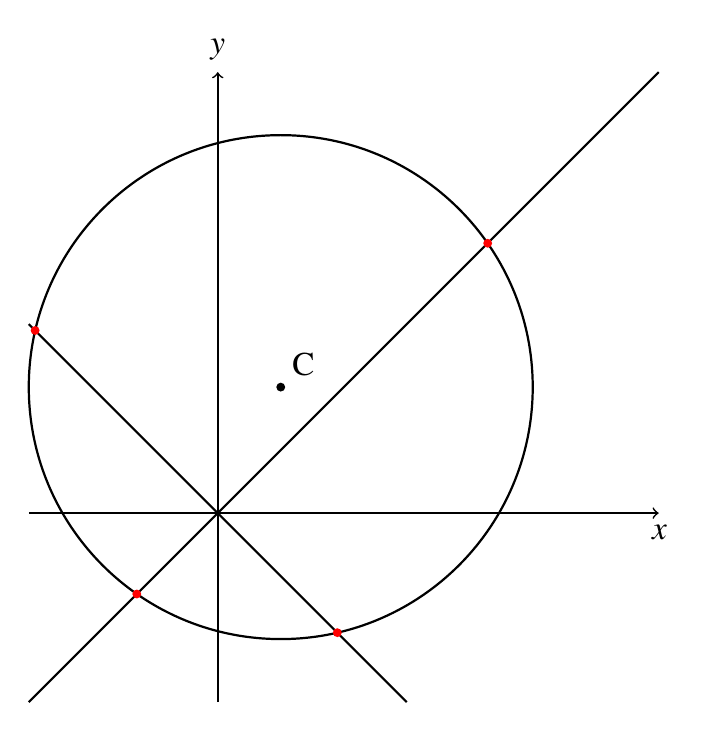
\begin{tikzpicture}[scale=0.8]\large
            \coordinate (c) at (1,2);
            \draw[semithick,->](-3,0)--(7,0)node[below]{\(x\)};
            \draw[semithick,->](0,-3)--(0,7)node[above]{\(y\)};
            \fill (c)node[above right]{C} circle (2pt);
            \draw[thick,name path=c_circ](c)circle[radius=4];
            \draw[thick,name path=p_x](-3,-3)--(7,7);
            \draw[thick,name path=m_x](-3,3)--(3,-3);

            \fill[name intersections={of=c_circ and p_x,by={p1,p2}},red] (p1) circle(2pt);
            \fill[red](p2)circle (2pt);
            \fill[name intersections={of=c_circ and m_x,by={m1,m2}},red] (m1) circle(2pt);
            \fill[red](m2)circle (2pt);

        \end{tikzpicture}
        \caption{問題の結果}
        \label{tikz_vector_equation_example_question}
    \end{figure}


    この例からもわかる通り,ベクトル方程式は求めたいベクトルの条件を与えるために用いられる.そのため,"方程式"なのだ.
    そして,これは無意識のうちになされることが多く,さらには条件の与え方を方程式という形ではなく,ベクトルの成分として
    \footnote{本問では,容易に \(y=\pm x\)が得られるので,計算をする前から \(\vec{p}=(x,x),(x,-x)\)とおいて, \(x\)についての計算問題とするほうが自然だ.}
    与えるケースが多い.そのため,優先度の低い事柄となっている.発想としては重要なものであるのでマスターしたい.\\

    ベクトル方程式の章では問題を用意しない.これまでの問題や,問題集の問題をベクトル方程式を用いて解くことで復習してほしい.

    \section*{まとめ}
    数B:ベクトルの内容を計算,図形,方程式という3つの側面から扱った.その中でもベクトルの有効性を発揮するために重要なのは,内積などの特別な計算規則を身につけることだ.ベクトルという大きさと向きを持つ量が,計算規則に従うことであたかも文字式のように扱えるようになることが極めて重要なことである.

    図形では,本来3つの要素を取り扱わなければならない3次元の問題に対しても代数的な計算を実現している.これがベクトルの最大の利点である.しかし,いかなる状況でもベクトルが有効なのではなく,角度や大きさが前面に出る問題では計算を実行できないというケースが存在するので,使いどころには注意が必要だ.これに関しては,反復練習のみが有効な訓練となる.

    最後のベクトル方程式はベクトルを図形に反映させるための1通りの手法ととらえると,良いだろう.ベクトルを求めるときに,ベクトルの成分を未知数として考えるのは良くない.それは単なる計算問題となってしまう.しかし,ベクトル方程式を立て,未知のベクトルを直接求めようとすれば,さらにベクトルの有効性を体感するに至るだろう.











\end{document}
